\documentclass[aspectratio=169]{beamer}
\usepackage[utf8]{inputenc}
\usepackage[T1]{fontenc}
\usepackage[spanish,es-tabla]{babel}
\usepackage{booktabs,graphicx,tikz,amsmath,adjustbox}
\usetikzlibrary{arrows.meta,positioning}
\usepackage{tesis_beamer}

% Versión de predefensa (10 láminas + anexo). Figuras: las del paper (especificación vigente) y, como respaldo, las de la tesis.
% En el zip para Prism todas viven en imagenes/. Las baterías se cargan desde tablas/
% (generadas por tablas_beamer.py a partir de las tablas de la tesis).
\graphicspath{{../envios/paper_empirico/figuras/}{../tesis/imagenes/}{imagenes/}}

% Una sola tabla de contenidos al inicio: sin la recapitulación automática por sección
\AtBeginSection[]{}

% Notación compartida con la tesis
\newcommand{\JLoss}{\mathrm{JLoss}}
\newcommand{\GaR}{\mathrm{GaR}}
\newcommand{\Spread}{\mathrm{spread}}
\newcommand{\EMBI}{\mathrm{EMBI}}
% Cifra destacada
\newcommand{\cifra}[2]{\begin{center}{\Huge\bfseries\color{tesisblue}#1}\\[2pt]{\small #2}\end{center}}
% Leyenda común de las baterías
\newcommand{\notabat}[1]{\par\vspace{3pt}{\scriptsize\raggedright
\textbf{Cómo leer:} variable dependiente $\ln\EMBI_{i,t}$. #1
Efectos fijos: P = país, T = tiempo (trimestre), PT = ambos. Ref.\ = especificación de referencia con EF país + tiempo.
Errores Driscoll--Kraay; *** $p<0{,}01$, ** $p<0{,}05$, * $p<0{,}10$. Celda vacía: la variable no está en ese modelo.\par}}

\author{Mauricio Valenzuela Corvalán}
\institute[Universidad de Chile]{Departamento de Ingeniería Civil Industrial\\
\small Magíster en Economía Aplicada · Universidad de Chile}
\title[Fragilidad bancaria y riesgo de cola]{Fragilidad bancaria sistémica y riesgo de cola del crecimiento}
\subtitle{Determinantes del \textit{spread} soberano en economías emergentes}
\date{\today}

\setbeamertemplate{navigation symbols}{}

\begin{document}

% =====================================================================
% 1
\begin{frame}
\titlepage
\vspace{-8pt}
\centering
\footnotesize Profesor guía: Juan Francisco Martínez Sepúlveda \quad\quad
Profesor coguía: Ronald Fischer
\end{frame}

% 2
\section{Pregunta}
\begin{frame}{La pregunta: dos riesgos domésticos de cola y el \textit{spread} soberano}
\begin{exampleblock}{\textit{Spread} soberano}
\footnotesize Prima que exige el mercado por el riesgo de incumplimiento de un gobierno emergente: rendimiento de su deuda en dólares menos el del Tesoro de EE.UU.\ (EMBI, en puntos básicos).
\end{exampleblock}
\vspace{-8pt}
\begin{columns}[T]
\column{0.48\textwidth}
\begin{block}{Riesgo financiero}
\footnotesize Fragilidad del sistema bancario: $\JLoss$. Chari et al.\ (2024) ya documentan que se asocia con el \textit{spread}.
\end{block}
\column{0.48\textwidth}
\begin{block}{Riesgo económico}
\footnotesize Cola adversa del crecimiento: $\GaR$ (Adrian et al., 2019). No se ha cruzado con la fragilidad.
\end{block}
\end{columns}
\begin{alertblock}{Brecha y pregunta}
\footnotesize No se han cruzado \textbf{simultáneamente} los dos riesgos de cola domésticos. Sobre la fragilidad bancaria, ¿\textbf{qué agrega} el riesgo económico, y qué pasa cuando los dos \textbf{se dan a la vez}?
\end{alertblock}
\end{frame}

% 3
\section{Mecanismo e hipótesis}
\begin{frame}{El mecanismo: un triángulo, no una secuencia}
\begin{columns}[c]
\column{0.6\textwidth}
\centering
\resizebox{\textwidth}{!}{%
\begin{tikzpicture}[
  box/.style={draw, thick, rounded corners, align=center, fill=gray!7,
              text width=3.9cm, minimum height=1.15cm, font=\small},
  boxhi/.style={box, draw=tesisblue, fill=tesisblue!8, line width=1pt},
  lbl/.style={font=\scriptsize\itshape, align=center}
]
\node[box]   (jloss)  at (0,0)    {Riesgo financiero:\\ fragilidad bancaria ($\JLoss$)};
\node[box]   (gar)    at (8.8,0) {Riesgo económico:\\ cola del crecimiento ($\GaR$)};
\node[boxhi] (spread) at (4.4,-3.2) {\textit{Spread} soberano (EMBI)};
\draw[thick] (jloss) -- (gar)
  node[midway, above, lbl, text width=4.2cm] {menos crédito, menor crecimiento (acelerador financiero)}
  node[midway, below, lbl, text width=4.2cm] {el crecimiento débil deteriora a los bancos};
\draw[-{Latex[length=2.4mm]}, tesisblue, line width=0.9pt] (jloss) -- (spread)
  node[midway, left, lbl, text width=2.6cm] {rescate esperado (pasivo contingente)};
\draw[-{Latex[length=2.4mm]}, tesisblue, line width=0.9pt] (gar) -- (spread)
  node[midway, right, lbl, text width=2.6cm] {capacidad fiscal en la cola};
\draw[-{Latex[length=2.4mm]}, dashed, gray!50!black]
  (spread.west) to[bend left=35] node[midway, left, lbl, text width=2.2cm] {retroalimentación} (jloss.south west);
\end{tikzpicture}%
}
{\scriptsize Bernanke, Gertler y Gilchrist (1996); Farhi y Tirole (2018); Acharya et al.\ (2014).}
\column{0.38\textwidth}
\begin{block}{¿Qué podría contenerla?}
\footnotesize
\begin{itemize}
\item Respaldo oficial: \textbf{banco central} (reservas) y líneas externas.
\item Quién tiene la deuda.
\end{itemize}
Se contrastan: reservas, acceso por país y participación extranjera.
\end{block}
\begin{alertblock}{Alcance}
\footnotesize Asociaciones, no causalidad: las tres cosas ocurren a la vez.
\end{alertblock}
\end{columns}
\end{frame}

% 4
\begin{frame}{Hipótesis de trabajo}
\begin{enumerate}
\item \textbf{H1 (canal bancario).} La fragilidad bancaria sistémica eleva el \textit{spread} soberano.
\vspace{4pt}
\item \textbf{H2 (canal de crecimiento).} Un mayor riesgo de cola del crecimiento eleva el \textit{spread} soberano.
\vspace{4pt}
\item \textbf{H3 (amplificación).} La coincidencia de ambos riesgos eleva el \textit{spread} más que la suma de las dos asociaciones.
\end{enumerate}
Además se contrasta si tres condiciones ---resiliencia, respaldo externo y quién tiene la deuda--- modifican la transmisión.
\end{frame}

% 5
\section{Datos y metodología}
\begin{frame}{Las dos variables en el tiempo}
\centering
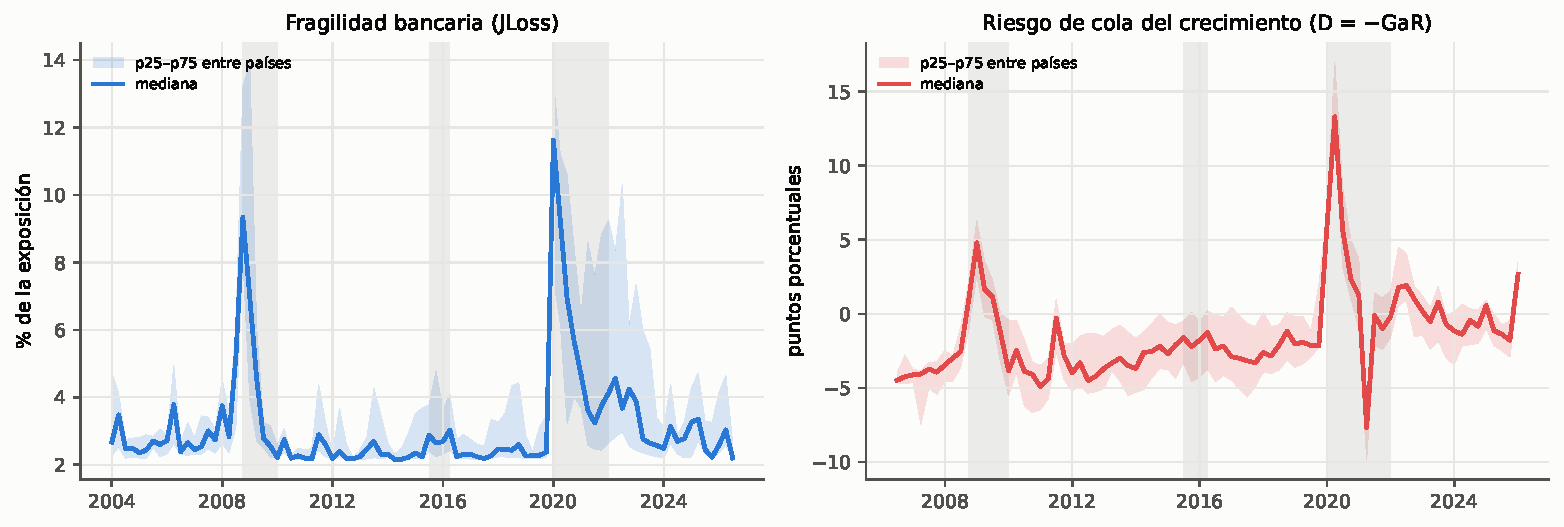
\includegraphics[width=0.95\textwidth,height=0.62\textheight,keepaspectratio]{fig_series_agregadas_embiext.pdf}\\
\footnotesize Mediana y rango p25--p75 entre las 13 economías del panel; sombreado: crisis financiera global, estrés emergente de 2015--16 y pandemia. Ambas saltan en las crisis. $\JLoss$: 113 bancos (Bloomberg), pérdida conjunta esperada del sistema. $D=-\GaR$: cuantil 5\% del crecimiento, con signo invertido.
\end{frame}

% 6
\begin{frame}{Metodología}
\begin{block}{Especificación principal (panel trimestral, 13 economías, 2004--2026, $N=765$)}
\small
\vspace{-6pt}
\[
\ln\EMBI_{i,t}=\alpha_i+\delta_t+\beta_1\ln\JLoss_{i,t-1}+\beta_2D_{i,t-1}+\beta_3\,(\ln\JLoss\times D)_{i,t-1}+\varepsilon_{i,t}
\]
\vspace{-8pt}
\end{block}
{\scriptsize \textbf{Donde:} $i$ país, $t$ trimestre; $\alpha_i$, $\delta_t$ efectos fijos de país y de tiempo; $D=-\GaR$ riesgo de cola; $\beta_1$, $\beta_2$ asociación de cada riesgo con el \textit{spread}; $\beta_3$ interacción ($>0$: amplificación; $=0$: efectos aditivos).\par}
\vspace{4pt}
\small
\begin{itemize}
\item \textbf{Rezagos} de un trimestre y \textbf{efectos fijos de tiempo}, que absorben los factores globales.
\item \textbf{Inferencia calibrada por simulación}: en niveles el criterio es el \textit{wild cluster bootstrap} por país; Driscoll--Kraay rechaza de más.
\item \textbf{Prueba preespecificada}: la participación extranjera se contrastó con hipótesis fijadas antes de estimar y corrección de Holm.
\item \textbf{Además}: permutación, cambios, proyecciones locales y pronóstico fuera de muestra.
\end{itemize}
\end{frame}

% 7
\section{Resultados}
\begin{frame}{Resultado 1: los dos riesgos coinciden más de lo que explicaría el azar}
\centering
\footnotesize
\begin{adjustbox}{max width=\textwidth}
\begin{tabular}{l ccc}
\toprule
\textit{Ambos riesgos en su tercil alto (definido dentro de cada país)} & Observado & Por azar & $p$ \\
\midrule
Observaciones conjuntas ($22{,}0\%$ de 765) & \textbf{168} & 87 (independencia) & 1,9 veces (neto del calendario común: 132 esperadas, 1,3 veces) \\
Permutación por bloques dentro de cada país (999 réplicas) & 168 & $85{,}7$ & $0{,}001$ \\
Fuera de los trimestres de crisis & 108 & $59{,}3$ & $0{,}001$ \\
Duración media de los 62 episodios conjuntos (trimestres) & $2{,}71$ & $1{,}85$ & $0{,}003$ \\
Países con más coincidencias que las esperadas & \textbf{13 de 13} & & \\
\midrule
\textit{Rezago cruzado (rezago propio, EF de país y de tiempo)} & Coeficiente & & $p$ \textit{wild} \\
\midrule
Fragilidad en $t-1$ $\to$ riesgo de cola en $t$ & $\mathbf{0{,}405^{***}}$ & & $0{,}024$ \\
Riesgo de cola en $t-1$ $\to$ fragilidad en $t$ & $-0{,}006$ & & $0{,}48$ \\
\bottomrule
\end{tabular}
\end{adjustbox}
\vspace{-2pt}
\begin{columns}[T]
\column{0.56\textwidth}
\begin{block}{Lectura}
\footnotesize \textbf{Simultaneidad: firme.} Casi el doble de lo esperado, en todos los países y por más tiempo. \textbf{Precedencia: sugerente.} La fragilidad antecede al riesgo de cola y no al revés; descansa en un rezago trimestral.
\end{block}
\column{0.42\textwidth}
\begin{alertblock}{Salvedad}
\footnotesize Pocos episodios comunes: 129 de las 168 son de 2020 en adelante; el exceso sobre lo esperado viene de 2015--19 y 2023--26.
\end{alertblock}
\end{columns}
\end{frame}

% 8
\begin{frame}{Resultado 2: cuando coinciden, no hay evidencia de que se amplifiquen}
\centering
\footnotesize
\begin{adjustbox}{max width=\textwidth}
\begin{tabular}{l cc}
\toprule
Prueba & Estimación & $p$ \textit{wild bootstrap} \\
\midrule
Interacción $\beta_3$ de la regresión principal & $-0{,}011$ & $0{,}89$ \\
Estrés conjunto: extra con los dos riesgos altos (fragilidad alta $+0{,}091$; cola alta $+0{,}186$) & $-0{,}077$ & $0{,}23$ \\
Estrés conjunto uno a cuatro trimestres adelante & $-0{,}097$ a $-0{,}046$ & $0{,}17$ a $0{,}37$ \\
Forma funcional intermedia (Box--Cox, $\lambda=0{,}44$): interacción & $t=-0{,}19$ & $0{,}97$ \\
\bottomrule
\end{tabular}
\end{adjustbox}
\vspace{-3pt}
\begin{block}{Las bandas: cuánta amplificación no se puede descartar}
\footnotesize Con ambos riesgos una desviación estándar sobre su media, la suma de los dos es $+16{,}4\%$ de \textit{spread} (28 pb). El extra estimado es $-2{,}1$ puntos (en pb, $+3{,}0$). Lo máximo que admite el intervalo de 95\%: $+0{,}5$ (Driscoll--Kraay), $+2{,}9$ (\textit{wild}), $+5{,}3$ puntos (\textit{cluster}, 29\% de la suma); en pb, $+11$ sobre 28 (39\%).
\end{block}
\vspace{-2pt}
\begin{alertblock}{Lectura}
\footnotesize \textbf{No hay evidencia de amplificación}; los datos no permiten descartar un extra de hasta un 30--40\% de la suma.
\end{alertblock}
\vspace{-2pt}
{\scriptsize\raggedright Aditivo en logaritmos es proporcional en puntos básicos: es álgebra de la forma funcional, no un hallazgo. El signo negativo de $\beta_3$ es de Polonia (sin ella $+0{,}008$): no se lee como atenuación.\par}
\end{frame}

% 9
\begin{frame}{Resultados 3 y 4: el riesgo económico agrega poco; ninguna condición cambia la transmisión}
\begin{columns}[T]
\column{0.5\textwidth}
\centering
\footnotesize
\begin{adjustbox}{max width=\textwidth}
\begin{tabular}{l c}
\toprule
\multicolumn{2}{l}{\textit{Agregar el riesgo de cola al modelo de Chari et al.\ ($N=662$)}} \\
\midrule
$\beta_2$ ($p$ \textit{wild} $0{,}066$) & $0{,}037^{***}$ \\
Prueba conjunta $\beta_2=\beta_3=0$, $p$ \textit{wild} & $\mathbf{0{,}041}$ \\
$R^2$ dentro del país (base $\to$ con $D$ $\to$ con interacción) & $0{,}153\to0{,}185\to0{,}194$ \\
\midrule
\multicolumn{2}{l}{\textit{Pero}} \\
\midrule
Cambios a cuatro trimestres ($p$ \textit{wild} $0{,}13$) & $0{,}004$ \\
Proyecciones locales, horizontes significativos & 0 de 9 \\
Fuera de muestra: error de pronóstico (evidencia débil) & $+3\%$ \\
Sin Polonia ($p=0{,}51$) & $0{,}007$ \\
\bottomrule
\end{tabular}
\end{adjustbox}

\vspace{3pt}
{\scriptsize\raggedright Una asociación modesta, de un 2--3\,\% de \textit{spread} por punto de riesgo de cola, en niveles y en 10 de 13 países. Evidencia \textbf{sugerente}: el \textit{wild bootstrap} no protege del sesgo de retroalimentación.\par}
\column{0.48\textwidth}
\begin{block}{¿Alguna condición la cambia?}
\footnotesize
\begin{itemize}\setlength\itemsep{2pt}
\item \textbf{Participación extranjera} en la deuda (preespecificada): $+0{,}037$, $-0{,}001$ y $-0{,}006$; Holm $p=1{,}00$. \textbf{No} (en pb, un indicio).
\item \textbf{Respaldo externo} por país (\textit{swap} de la Fed, línea flexible del FMI): $-0{,}004$ ($p$ \textit{wild} $0{,}90$). \textbf{No.}
\item \textbf{Reservas} $\times$ fragilidad: $-0{,}247$ ($p$ \textit{wild} $0{,}08$; Holm $0{,}40$); en logaritmos depende de Polonia y otras variables dan lo mismo. \textbf{Exploratorio.}
\end{itemize}
\end{block}
\end{columns}
\end{frame}

% 10
\section{Conclusiones}
\begin{frame}{Conclusiones e implicancias}
\small
\begin{enumerate}\setlength\itemsep{1pt}
\item \textbf{La simultaneidad es un hecho} (firme): los dos riesgos coinciden 1,9 veces lo esperado por azar (1,3 neto); hay indicios (sugerente) de que la fragilidad antecede al riesgo de cola.
\item \textbf{Cuando coinciden, no hay evidencia de que se amplifiquen}; no se descarta un extra de hasta un 30--40\% de la suma.
\item \textbf{El riesgo económico agrega poco} (sugerente): solo en niveles; no mejora el pronóstico.
\item \textbf{Ninguna condición} ---resiliencia, respaldo externo, quién tiene la deuda--- modifica la transmisión de forma demostrable.
\end{enumerate}
{\footnotesize \textbf{Réplica:} la asociación fragilidad--\textit{spread} replica a Chari et al.\ con sus controles, pero no es una elasticidad común ni hay precedencia temporal.\par}
\vspace{-2pt}
\begin{block}{Implicancias}
\footnotesize Vigilar los dos riesgos juntos se justifica: tienden a agravarse a la vez. No hay base para una prima adicional por la simultaneidad, ni para recomendar reservas o diferenciar por quién tiene la deuda. No se puede cuantificar cuánto bajaría el \textit{spread} si cae la fragilidad.
\end{block}
\end{frame}

% =====================================================================
\appendix
\section{Anexos}

\begin{frame}{Anexo: Construcción de $\JLoss$: fragilidad bancaria sistémica}
\small
Pérdida conjunta esperada del sistema bancario ante un evento sistémico, en \% de la exposición (Chari et al., 2024).
\begin{enumerate}
\item \textbf{Probabilidad de incumplimiento de cada banco} (Merton--KMV): $D^*=L_{ST}+\tfrac12L_{LT}$,\quad $EDF=\Phi(-DD)$.
\item \textbf{Factor sistémico} país (Vasicek): $p_i(V)=\Phi\!\left(\frac{\Phi^{-1}(p_i)-\rho_iV}{\sqrt{1-\rho_i^2}}\right)$.
\item \textbf{Agregación por punto de silla} de la distribución de pérdidas del sistema.
\item \textbf{Métrica}: $\JLoss=\dfrac{EL+UL}{\sum_j EAD_j}\times100$.
\end{enumerate}
\vspace{2pt}
{\scriptsize \textbf{Donde:} $D^*$ punto de incumplimiento; $L_{ST}$, $L_{LT}$ pasivos de corto y largo plazo; $DD$ distancia al incumplimiento; $EDF$ frecuencia esperada de incumplimiento; $\Phi$ distribución normal estándar; $p_i$ PD del banco $i$; $V$ factor sistémico (retorno bursátil del país); $\rho_i$ correlación del banco con $V$; $EL$ pérdida esperada; $UL$ pérdida inesperada al 99\%; $EAD$ exposición; LGD $=45\%$. La cota de la malla es activa en el 98\% de los casos $\Rightarrow$ $\JLoss$ es \textbf{ordinal} y entra en logaritmos.\par}
\end{frame}

\begin{frame}{Anexo: Construcción del $\GaR$: riesgo de cola del crecimiento}
\begin{columns}[c]
\column{0.52\textwidth}
\footnotesize
\begin{enumerate}
\item \textbf{Índice de condiciones financieras} (FCI tipo CISS): tensión accionaria, de tasas y cambiaria, en términos reales (deflactadas por la inflación).
\item \textbf{Regresión cuantílica de panel}, un trimestre adelante:\\
{\footnotesize $Q(\Delta y_{i,t+1}\mid\cdot;\tau)=\alpha+\beta_1\Delta y_{i,t}+\beta_2FCI^{\perp}_{i,t}+\beta_3VIX_t+\mu_i$}
\item $\GaR_{i,t}$ = cuantil $\tau=5\%$; ventana expansiva (pseudo--tiempo real).
\end{enumerate}
\vspace{2pt}
{\scriptsize \textbf{Donde:} $Q(\cdot;\tau)$ cuantil $\tau$ del crecimiento; $\Delta y$ crecimiento del PIB; $FCI^{\perp}$ FCI sin el componente del VIX; $\mu_i$ efecto fijo de país. En la tesis $D\equiv-\GaR$: mayor $D$, cola más adversa. No es circular con el EMBI (corr.\ 0,985 sin el componente tipo \textit{spread}).\par}
\column{0.46\textwidth}
\centering
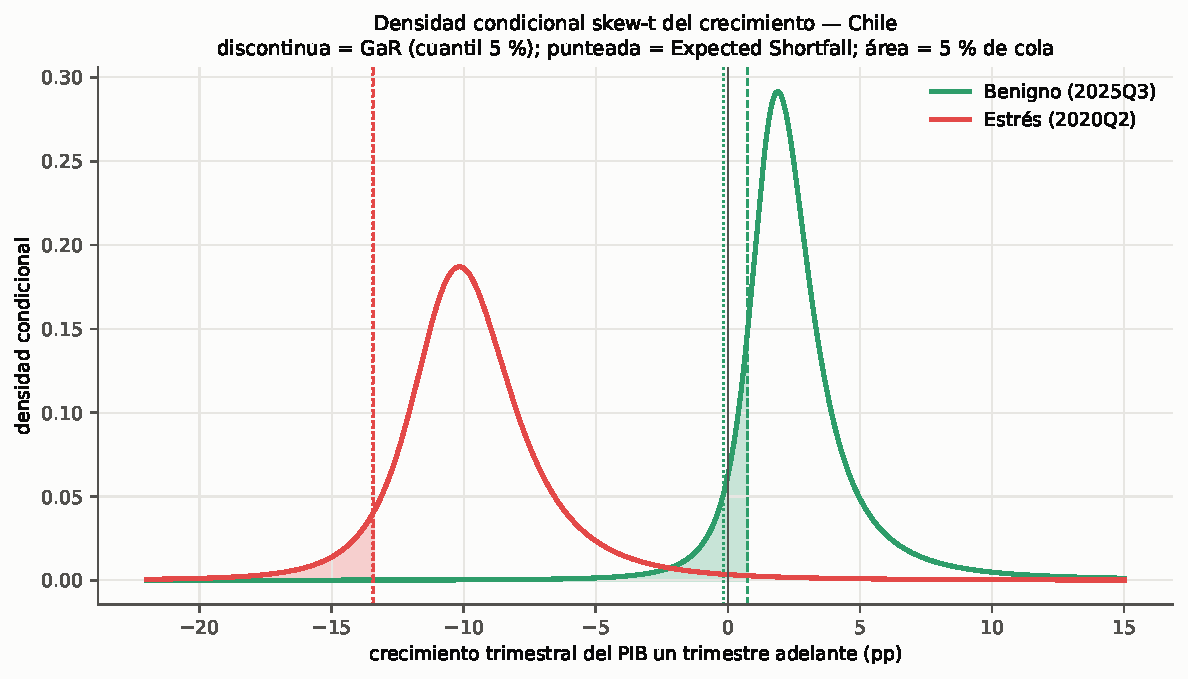
\includegraphics[width=\textwidth]{fig_skewt_chile_embiext.pdf}\\
{\scriptsize Chile: trimestre benigno vs.\ 2020Q2 ($\GaR=-13{,}4$ pp).}
\end{columns}
\end{frame}

\begin{frame}{Anexo: Batería principal · Panel A: muestra completa}
\centering
\small
% Generado por tablas_beamer.py a partir de las tablas de la tesis; no editar a mano.
\begingroup\setlength{\tabcolsep}{3pt}\renewcommand{\arraystretch}{1.3}%
\begin{adjustbox}{max width=0.97\textwidth}
\begin{tabular}{l c ccc ccc ccc cc}
\toprule
 & Ref. & \multicolumn{3}{c}{M1} & \multicolumn{3}{c}{M2} & \multicolumn{3}{c}{M3} & \multicolumn{2}{c}{M4} \\
\cmidrule(lr){2-2}\cmidrule(lr){3-5}\cmidrule(lr){6-8}\cmidrule(lr){9-11}\cmidrule(lr){12-13}
Efectos fijos & PT & T & P & PT & T & P & PT & T & P & PT & T & P \\
 & (1) & (2) & (3) & (4) & (5) & (6) & (7) & (8) & (9) & (10) & (11) & (12) \\
\midrule
Fragilidad, $\beta_1$ & $0{,}099^{***}$ & $0{,}198^{***}$ & $0{,}196^{***}$ & $0{,}127^{***}$ &  &  &  & $0{,}242^{***}$ & $0{,}152^{***}$ & $0{,}097^{***}$ & $0{,}245^{***}$ & $0{,}152^{***}$ \\
Riesgo de cola, $\beta_2$ & $0{,}032^{**}$ &  &  &  & $0{,}044^{***}$ & $0{,}028^{***}$ & $0{,}037^{**}$ & $0{,}053^{***}$ & $0{,}015^{*}$ & $0{,}030^{*}$ & $0{,}055^{***}$ & $0{,}017^{*}$ \\
\textbf{Interacción}, $\beta_3$ & $-0{,}011$ &  &  &  &  &  &  &  &  &  & $-0{,}016$ & $-0{,}006$ \\
\addlinespace
Observaciones & 765 & 765 & 765 & 765 & 765 & 765 & 765 & 765 & 765 & 765 & 765 & 765 \\
\bottomrule
\end{tabular}
\end{adjustbox}\endgroup

\notabat{M1 solo fragilidad; M2 solo riesgo de cola; M3 ambos; M4 ambos con interacción. $\beta_1$ elasticidad a $\ln\JLoss_{t-1}$; $\beta_2$ semielasticidad a $D_{t-1}=-\GaR_{t-1}$; $\beta_3$ interacción. Sin controles.}
\end{frame}

\begin{frame}{Anexo: Batería principal · Panel B: sin trimestres de crisis}
\centering
\small
% Generado por tablas_beamer.py a partir de las tablas de la tesis; no editar a mano.
\begingroup\setlength{\tabcolsep}{3pt}\renewcommand{\arraystretch}{1.3}%
\begin{adjustbox}{max width=0.97\textwidth}
\begin{tabular}{l c ccc ccc ccc cc}
\toprule
 & Ref. & \multicolumn{3}{c}{M1} & \multicolumn{3}{c}{M2} & \multicolumn{3}{c}{M3} & \multicolumn{2}{c}{M4} \\
\cmidrule(lr){2-2}\cmidrule(lr){3-5}\cmidrule(lr){6-8}\cmidrule(lr){9-11}\cmidrule(lr){12-13}
Efectos fijos & PT & T & P & PT & T & P & PT & T & P & PT & T & P \\
 & (1) & (2) & (3) & (4) & (5) & (6) & (7) & (8) & (9) & (10) & (11) & (12) \\
\midrule
Fragilidad, $\beta_1$ & $0{,}087^{**}$ & $0{,}206^{***}$ & $0{,}182^{***}$ & $0{,}142^{***}$ &  &  &  & $0{,}259^{***}$ & $0{,}121^{***}$ & $0{,}086^{**}$ & $0{,}257^{***}$ & $0{,}120^{***}$ \\
Riesgo de cola, $\beta_2$ & $0{,}050^{***}$ &  &  &  & $0{,}056^{***}$ & $0{,}039^{***}$ & $0{,}058^{***}$ & $0{,}065^{***}$ & $0{,}027$ & $0{,}051^{***}$ & $0{,}063^{***}$ & $0{,}026$ \\
\textbf{Interacción}, $\beta_3$ & $0{,}005$ &  &  &  &  &  &  &  &  &  & $0{,}015$ & $0{,}009$ \\
\addlinespace
Observaciones & 656 & 656 & 656 & 656 & 656 & 656 & 656 & 656 & 656 & 656 & 656 & 656 \\
\bottomrule
\end{tabular}
\end{adjustbox}\endgroup

\notabat{Excluye 2008Q4--2009Q4 y 2020Q1--2021Q4. M1--M4 y $\beta_1$--$\beta_3$ como en el Panel A. Sin controles.}
\end{frame}

\begin{frame}{Anexo: Batería principal · Panel C: con seis controles domésticos}
\centering
\small
% Generado por tablas_beamer.py a partir de las tablas de la tesis; no editar a mano.
\begingroup\setlength{\tabcolsep}{3pt}\renewcommand{\arraystretch}{1.3}%
\begin{adjustbox}{max width=0.97\textwidth}
\begin{tabular}{l c ccc ccc ccc cc}
\toprule
 & Ref. & \multicolumn{3}{c}{M1} & \multicolumn{3}{c}{M2} & \multicolumn{3}{c}{M3} & \multicolumn{2}{c}{M4} \\
\cmidrule(lr){2-2}\cmidrule(lr){3-5}\cmidrule(lr){6-8}\cmidrule(lr){9-11}\cmidrule(lr){12-13}
Efectos fijos & PT & T & P & PT & T & P & PT & T & P & PT & T & P \\
 & (1) & (2) & (3) & (4) & (5) & (6) & (7) & (8) & (9) & (10) & (11) & (12) \\
\midrule
Fragilidad, $\beta_1$ & $-0{,}008$ & $0{,}004$ & $0{,}100$ & $0{,}004$ &  &  &  & $0{,}024$ & $0{,}062$ & $-0{,}013$ & $0{,}033$ & $0{,}072$ \\
Riesgo de cola, $\beta_2$ & $0{,}028^{**}$ &  &  &  & $0{,}013$ & $0{,}024^{**}$ & $0{,}026^{*}$ & $0{,}014$ & $0{,}021^{**}$ & $0{,}027^{*}$ & $0{,}017$ & $0{,}027^{***}$ \\
\textbf{Interacción}, $\beta_3$ & $-0{,}006$ &  &  &  &  &  &  &  &  &  & $-0{,}014$ & $-0{,}014^{**}$ \\
\addlinespace
Observaciones & 649 & 649 & 649 & 649 & 649 & 649 & 649 & 649 & 649 & 649 & 649 & 649 \\
\bottomrule
\end{tabular}
\end{adjustbox}\endgroup

\notabat{Agrega deuda/PIB, balance fiscal/PIB, reservas/PIB, cuenta corriente/PIB, inflación y tipo de cambio real. M1--M4 y $\beta_1$--$\beta_3$ como en el Panel A.}
\end{frame}

\begin{frame}{Anexo: Réplica de Chari et al.\ y sus límites}
\begin{columns}[c]
\column{0.56\textwidth}
\centering
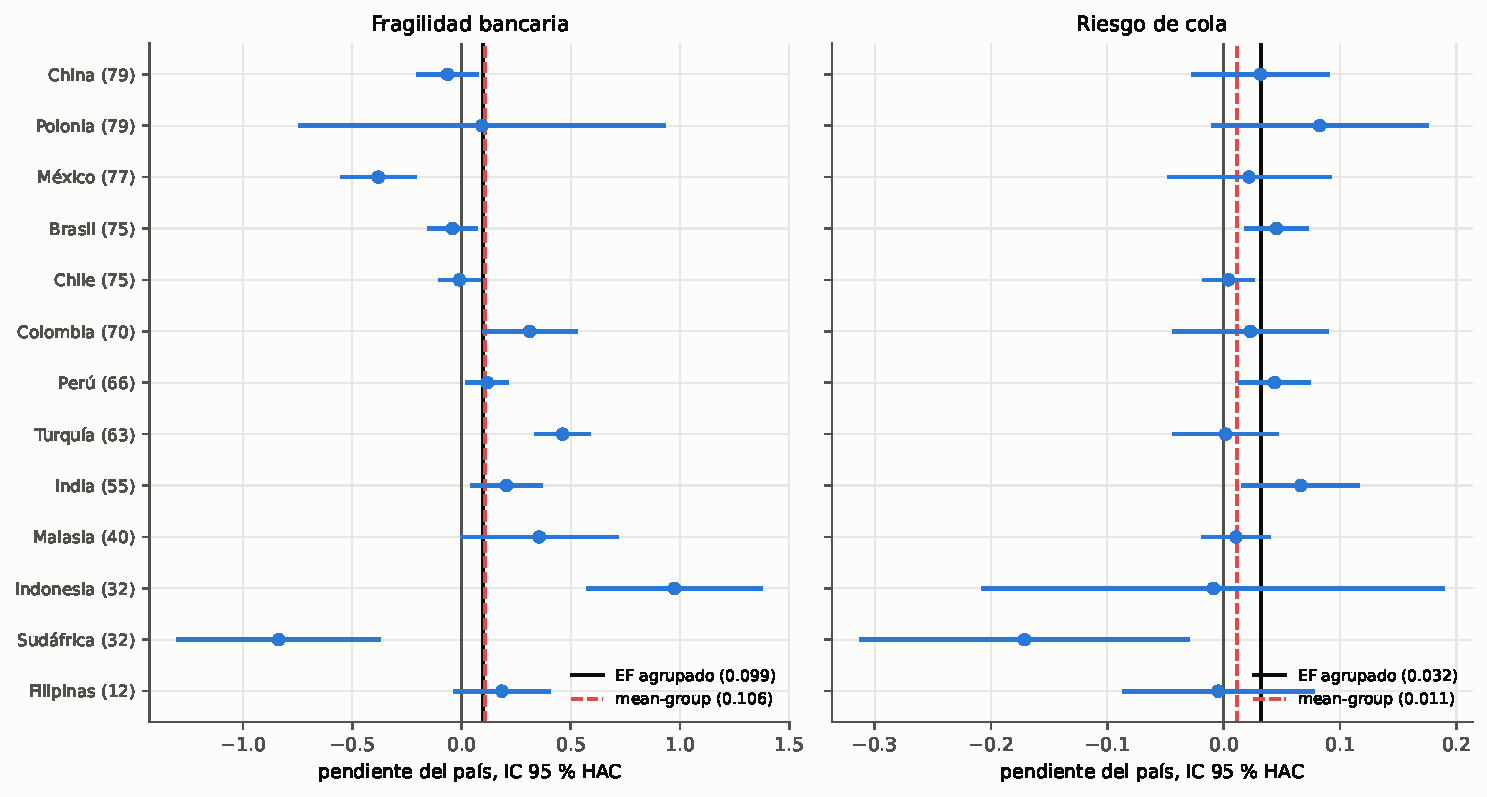
\includegraphics[width=\textwidth]{fig_pendientes_pais_lnlag.pdf}\\
{\scriptsize Pendiente de cada país, IC 95\%; entre paréntesis, sus trimestres.}
\column{0.43\textwidth}
\footnotesize
\begin{itemize}\setlength\itemsep{1pt}
\item \textbf{Se replica con sus controles}: $0{,}107$--$0{,}164$ ($0{,}206$ con el CDS). Con los seis controles domésticos de la tesis: $-0{,}008$.
\item \textbf{No es una elasticidad común}: pendientes entre $-0{,}84$ y $+0{,}97$; promedio de grupo $0{,}106$ ($p=0{,}39$); se rechaza la homogeneidad.
\item \textbf{Turquía} aporta el 70\% del coeficiente: sin ella, $0{,}034$ ($p=0{,}43$).
\item \textbf{Piso de $\JLoss$} (2,16): el 24\% de las observaciones está pegado al piso; ahí la métrica no informa.
\item Una desviación estándar dentro del país $\approx+5\%$ de \textit{spread} (13 pb).
\end{itemize}
\end{columns}
\end{frame}

\begin{frame}{Anexo: Fechas: la fragilidad y el \textit{spread} se mueven en el mismo trimestre}
\centering
\footnotesize
\begin{adjustbox}{max width=\textwidth}
\begin{tabular}{l cc cc}
\toprule
 & \multicolumn{2}{c}{Logaritmos} & \multicolumn{2}{c}{Puntos básicos} \\
\cmidrule(lr){2-3}\cmidrule(lr){4-5}
Cambio del \textit{spread} sobre el cambio de la fragilidad en $t-1$ ($N=708$) & Coef. & $p$ \textit{wild} & Coef. & $p$ \textit{wild} \\
\midrule
Promedio de $t$ menos promedio de $t-1$ (la versión de la primera ronda) & $0{,}039^{***}$ & $<0{,}001$ & $1{,}30^{***}$ & $0{,}05$ \\
\textbf{Cierre de $t$ menos cierre de $t-1$} (prueba limpia de precedencia) & $\mathbf{0{,}025}$ & $0{,}21$ & $0{,}28$ & $0{,}58$ \\
Primer mes de $t$ menos cierre de $t-1$ & $0{,}000$ & $0{,}99$ & $0{,}04$ & $0{,}91$ \\
Cierre de $t-1$ menos promedio de $t-1$ (parte mecánica) & $0{,}020^{***}$ & $0{,}001$ & $1{,}03^{**}$ & $0{,}002$ \\
\textbf{Cierre de $t-1$ menos cierre de $t-2$} (mismo trimestre) & $\mathbf{0{,}037^{**}}$ & $0{,}008$ & $\mathbf{2{,}64^{***}}$ & $0{,}008$ \\
\bottomrule
\end{tabular}
\end{adjustbox}
\vspace{1pt}
\begin{itemize}\footnotesize\setlength\itemsep{0pt}
\item El EMBI del panel es el promedio diario del trimestre: la mitad del resultado en diferencias de la primera ronda (el 80\% en pb) era agregación temporal.
\item Con el \textit{spread} de cierre no hay precedencia: nunca es significativo al excluir un país o un año.
\item El movimiento en el mismo trimestre es robusto en pb (13 de 13 países, 23 de 23 años); en logaritmos, 6 de 13 y 13 de 23 (sin Turquía, $0{,}030$; $p=0{,}15$).
\end{itemize}
\vspace{-8pt}
\begin{alertblock}{Lectura}
\footnotesize Se mueven dentro del mismo trimestre; no hay evidencia de que la fragilidad anteceda al \textit{spread}. {\scriptsize (*** $p<0{,}01$, ** $p<0{,}05$, Driscoll--Kraay.)}
\end{alertblock}

\end{frame}

\begin{frame}{Anexo: ¿Efecto o persistencia? La retroalimentación}
\begin{columns}[c]
\column{0.55\textwidth}
\centering
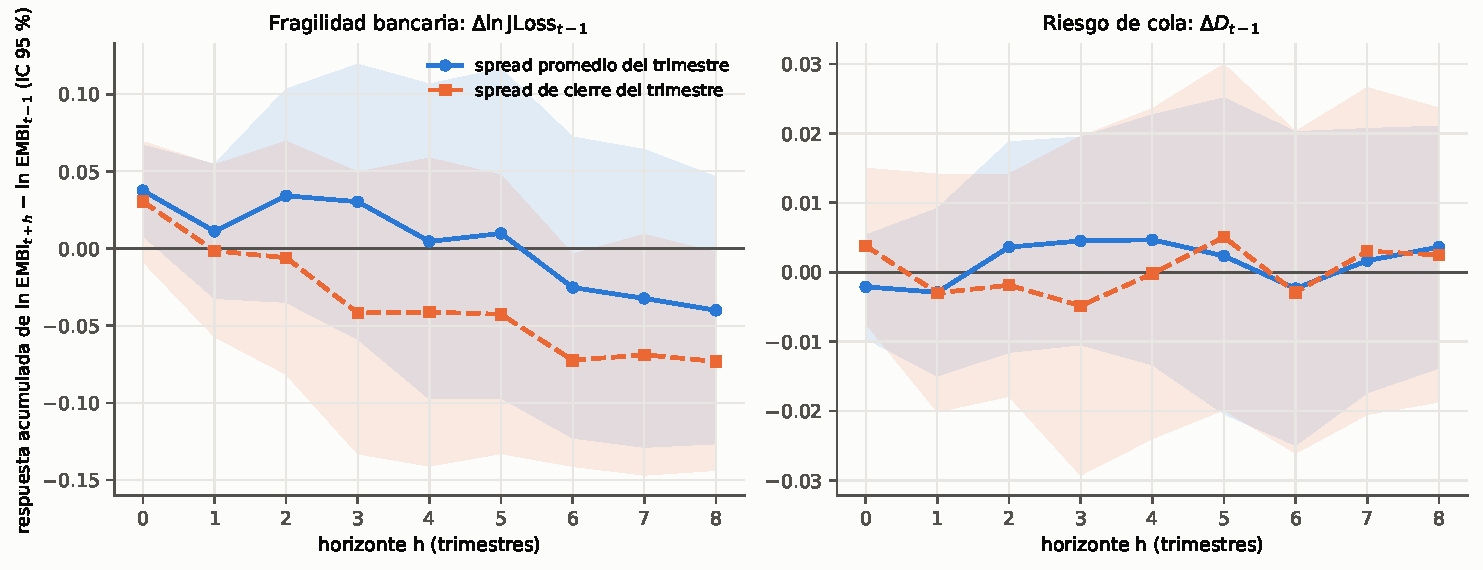
\includegraphics[width=\textwidth]{fig_lp_acumulada_lnlag.pdf}\\
{\scriptsize Proyecciones locales acumuladas: respuesta del \textit{spread} al cambio de la fragilidad (izq.) y del riesgo de cola (der.).}
\column{0.43\textwidth}
\footnotesize
\begin{itemize}\setlength\itemsep{2pt}
\item El \textit{spread} de ayer predice la fragilidad de hoy: \textbf{0,17} ($p=0{,}009$).
\item \textbf{Sesgo de retroalimentación}: en un panel simulado donde la fragilidad no tiene efecto directo, la regresión en niveles entrega $+0{,}066$ en promedio (dato: $0{,}099$). Para el riesgo de cola: $+0{,}022$ (dato: $0{,}032$).
\item \textbf{Nivel o cambio}: los datos no informan. Multiplicador de largo plazo $-0{,}146$, IC 95\% $[-0{,}79;\,0{,}50]$.
\item Proyecciones locales: solo el impacto con el \textit{spread} promedio ($0{,}038$); con el de cierre, nunca positiva y significativa. Riesgo de cola: plano.
\end{itemize}
\end{columns}
\end{frame}

\begin{frame}{Anexo: Inferencia calibrada por simulación}
\centering
\footnotesize
\begin{adjustbox}{max width=\textwidth}
\begin{tabular}{l ccc c}
\toprule
 & Tamaño (debería ser 5\%) & Potencia & Tamaño centrado, con retroalimentación & $p$ en los datos ($\beta_1$ / $\beta_2$ / $\beta_3$) \\
\midrule
\multicolumn{5}{l}{\textit{Niveles (fragilidad / riesgo de cola)}} \\
Driscoll--Kraay & $28\%$ / $21\%$ & $70\%$ / $77\%$ & $18\%$ / $18\%$ & $0{,}003$ / $0{,}033$ / $0{,}11$ \\
Driscoll--Kraay, banda larga y valores críticos \textit{fixed-b} & $15\%$ / $11\%$ & $56\%$ / $66\%$ & $9\%$ / $10\%$ & \\
\textit{Cluster} por país, $t(12)$ & $9\%$ / $8\%$ & $44\%$ / $70\%$ & $6\%$ / $14\%$ & $0{,}28$ / $0{,}14$ / $0{,}53$ \\
\textbf{\textit{Wild bootstrap} por país} & $\mathbf{6\%}$ / $\mathbf{7\%}$ & $35\%$ / $67\%$ & $5\%$ / $12\%$ & $0{,}33$ / $0{,}20$ / $0{,}89$ \\
\midrule
\multicolumn{5}{l}{\textit{Primeras diferencias}} \\
Driscoll--Kraay & $5\%$ / $6\%$ & $87\%$ (fragilidad) & & \\
\textit{Cluster} por país, $t(12)$ & $6\%$ / $9\%$ & $84\%$ & & \\
\textit{Wild bootstrap} por país & $6\%$ / $6\%$ & $81\%$ & & \\
\bottomrule
\end{tabular}
\end{adjustbox}
\vspace{2pt}
\begin{itemize}\footnotesize\setlength\itemsep{1pt}
\item 1\,000 paneles simulados que conservan la dependencia entre países; contraste al 5\%. En niveles, Driscoll--Kraay \textbf{rechaza de más}; en diferencias todos rechazan entre 5\% y 9\%.
\item El \textit{wild bootstrap} por país es el mejor calibrado, pero \textbf{no protege del sesgo de retroalimentación}: sin efecto directo, rechaza ``cero'' el 24\% de las veces (Driscoll--Kraay, 42--45\%).
\end{itemize}
\vspace{-6pt}
\begin{alertblock}{Regla de lectura}
\footnotesize En niveles, resistir el \textit{wild bootstrap} es necesario, no suficiente. Solo Driscoll--Kraay rechaza una hipótesis nula cierta entre el 20\% y el 30\% de las veces.
\end{alertblock}
\end{frame}

\begin{frame}{Anexo: Batería con vector de crisis · vector único}
\centering
\small
\begin{adjustbox}{max totalheight=0.62\textheight}
% Generado por tablas_beamer.py a partir de las tablas de la tesis; no editar a mano.
\begingroup\setlength{\tabcolsep}{3pt}\renewcommand{\arraystretch}{1.3}%
\begin{adjustbox}{max width=0.97\textwidth}
\begin{tabular}{l c ccc ccc ccc cc}
\toprule
 & Ref. & \multicolumn{3}{c}{CM1} & \multicolumn{3}{c}{CM2} & \multicolumn{3}{c}{CM3} & \multicolumn{2}{c}{CM4} \\
\cmidrule(lr){2-2}\cmidrule(lr){3-5}\cmidrule(lr){6-8}\cmidrule(lr){9-11}\cmidrule(lr){12-13}
Efectos fijos & PT & T & P & PT & T & P & PT & T & P & PT & T & P \\
 & (1) & (2) & (3) & (4) & (5) & (6) & (7) & (8) & (9) & (10) & (11) & (12) \\
\midrule
Fragilidad, $\beta_1$ & $-0{,}018$ & $0{,}003$ & $0{,}104^{*}$ & $-0{,}009$ &  &  &  & $0{,}028$ & $0{,}059$ & $-0{,}020$ & $0{,}029$ & $0{,}060$ \\
Riesgo de cola, $\beta_2$ & $0{,}037^{***}$ &  &  &  & $0{,}016$ & $0{,}046^{***}$ & $0{,}037^{***}$ & $0{,}017$ & $0{,}043^{***}$ & $0{,}037^{***}$ & $0{,}017$ & $0{,}043^{***}$ \\
\textbf{Interacción}, $\beta_3$ & $0{,}012$ &  &  &  &  &  &  &  &  &  & $0{,}001$ & $-0{,}002$ \\
Fragilidad $\times$ crisis & $0{,}040$ & $0{,}001$ & $-0{,}009$ & $0{,}042$ &  &  &  & $-0{,}007$ & $-0{,}002$ & $0{,}022$ & $0{,}041$ & $0{,}006$ \\
Riesgo de cola $\times$ crisis & $-0{,}017$ &  &  &  & $-0{,}010$ & $-0{,}034^{***}$ & $-0{,}026$ & $-0{,}011$ & $-0{,}033^{***}$ & $-0{,}025$ & $0{,}005$ & $-0{,}030^{**}$ \\
Interacción $\times$ crisis, $\beta_4$ & $-0{,}024^{*}$ &  &  &  &  &  &  &  &  &  & $-0{,}026$ & $-0{,}003$ \\
\textbf{Interacción en crisis}, $\beta_3+\beta_4$ & $-0{,}012^{**}$ &  &  &  &  &  &  &  &  &  & $-0{,}025^{***}$ & $-0{,}004$ \\
 & $[p=0{,}045]$ &  &  &  &  &  &  &  &  &  & $[p=0{,}004]$ & $[p=0{,}442]$ \\
\addlinespace
Observaciones & 649 & 649 & 649 & 649 & 649 & 649 & 649 & 649 & 649 & 649 & 649 & 649 \\
\bottomrule
\end{tabular}
\end{adjustbox}\endgroup

\end{adjustbox}
\notabat{CM1--CM4: modelos anidados con interacciones de crisis; todos con los seis controles. Crisis = 2008Q4--2009Q4, 2015Q3--2016Q1 y 2020Q1--2021Q4. $\beta_3$ interacción fuera de crisis; $\beta_4$ su cambio en crisis; $\beta_3+\beta_4$ interacción en crisis ($p$ entre corchetes).}
\end{frame}

\begin{frame}{Anexo: Batería con vector de crisis · \textit{Backstop} vs.\ \textit{EMstress}}
\centering
\small
\begin{adjustbox}{max totalheight=0.66\textheight}
% Generado por tablas_beamer.py a partir de las tablas de la tesis; no editar a mano.
\begingroup\setlength{\tabcolsep}{3pt}\renewcommand{\arraystretch}{1.3}%
\begin{adjustbox}{max width=0.97\textwidth}
\begin{tabular}{l c ccc ccc ccc cc}
\toprule
 & Ref. & \multicolumn{3}{c}{CM1} & \multicolumn{3}{c}{CM2} & \multicolumn{3}{c}{CM3} & \multicolumn{2}{c}{CM4} \\
\cmidrule(lr){2-2}\cmidrule(lr){3-5}\cmidrule(lr){6-8}\cmidrule(lr){9-11}\cmidrule(lr){12-13}
Efectos fijos & PT & T & P & PT & T & P & PT & T & P & PT & T & P \\
 & (1) & (2) & (3) & (4) & (5) & (6) & (7) & (8) & (9) & (10) & (11) & (12) \\
\midrule
Fragilidad, $\beta_1$ & $-0{,}019$ & $0{,}004$ & $0{,}103^{*}$ & $-0{,}009$ &  &  &  & $0{,}031$ & $0{,}056$ & $-0{,}022$ & $0{,}030$ & $0{,}056$ \\
Riesgo de cola, $\beta_2$ & $0{,}038^{***}$ &  &  &  & $0{,}016$ & $0{,}048^{***}$ & $0{,}038^{***}$ & $0{,}017$ & $0{,}045^{***}$ & $0{,}039^{***}$ & $0{,}017$ & $0{,}044^{***}$ \\
\textbf{Interacción}, $\beta_3$ & $0{,}013$ &  &  &  &  &  &  &  &  &  & $0{,}002$ & $-0{,}001$ \\
Fragilidad $\times$ \textit{Backstop} & $0{,}059$ & $-0{,}005$ & $-0{,}005$ & $0{,}059$ &  &  &  & $-0{,}030$ & $0{,}010$ & $0{,}037$ & $0{,}028$ & $0{,}021$ \\
Riesgo de cola $\times$ \textit{Backstop} & $-0{,}019$ &  &  &  & $-0{,}025$ & $-0{,}037^{***}$ & $-0{,}030$ & $-0{,}027$ & $-0{,}037^{***}$ & $-0{,}029$ & $-0{,}009$ & $-0{,}032^{**}$ \\
Interacción $\times$ \textit{Backstop}, $\beta_4^{bk}$ & $-0{,}027^{**}$ &  &  &  &  &  &  &  &  &  & $-0{,}031$ & $-0{,}006$ \\
Fragilidad $\times$ \textit{EMstress} & $-0{,}107^{***}$ & $0{,}028$ & $-0{,}037$ & $-0{,}033$ &  &  &  & $-0{,}015$ & $-0{,}066^{*}$ & $-0{,}073^{**}$ & $-0{,}059$ & $-0{,}110^{***}$ \\
Riesgo de cola $\times$ \textit{EMstress} & $-0{,}023$ &  &  &  & $0{,}053^{***}$ & $-0{,}003$ & $-0{,}008$ & $0{,}052^{***}$ & $-0{,}003$ & $-0{,}006$ & $0{,}027$ & $-0{,}028^{***}$ \\
Interacción $\times$ \textit{EMstress}, $\beta_4^{em}$ & $0{,}013$ &  &  &  &  &  &  &  &  &  & $0{,}034$ & $0{,}037^{**}$ \\
\textbf{Bajo \textit{Backstop}}, $\beta_3+\beta_4^{bk}$ & $-0{,}015^{**}$ &  &  &  &  &  &  &  &  &  & $-0{,}029^{***}$ & $-0{,}007$ \\
 & $[p=0{,}030]$ &  &  &  &  &  &  &  &  &  & $[p=0{,}001]$ & $[p=0{,}293]$ \\
\textbf{Bajo \textit{EMstress}}, $\beta_3+\beta_4^{em}$ & $0{,}026^{*}$ &  &  &  &  &  &  &  &  &  & $0{,}036^{**}$ & $0{,}036^{***}$ \\
 & $[p=0{,}080]$ &  &  &  &  &  &  &  &  &  & $[p=0{,}043]$ & $[p=0{,}001]$ \\
\addlinespace
Observaciones & 649 & 649 & 649 & 649 & 649 & 649 & 649 & 649 & 649 & 649 & 649 & 649 \\
\bottomrule
\end{tabular}
\end{adjustbox}\endgroup

\end{adjustbox}
\notabat{\textit{Backstop} = GFC (2008Q4--2009Q4) y COVID (2020Q1--2021Q4), con respaldo oficial a escala global; \textit{EMstress} = 2015Q3--2016Q1, sin respaldo. $\beta_4^{bk}$, $\beta_4^{em}$ cambios de la interacción en cada episodio. Todos con los seis controles.}
\end{frame}

\begin{frame}{Anexo: Lectura: el patrón esperado, pero sin robustez}
\begin{columns}[c]
\column{0.5\textwidth}
\footnotesize
\begin{itemize}
\item Fuera de crisis: $\beta_3$ entre $-0{,}002$ y $+0{,}013$ (nulo).
\item \textit{Backstop}: $-0{,}015$ ($p=0{,}03$).
\item \textit{EMstress}: $+0{,}026$ ($p=0{,}08$).
\item \textbf{Al pie de la letra}, el patrón del mecanismo.
\end{itemize}
\vspace{2pt}
\begin{alertblock}{Pero}
\footnotesize
\begin{itemize}
\item Corrección de Holm: $p=0{,}12$ y $p=0{,}24$.
\item \textit{Cluster} por país: $p=0{,}40$ y $p=0{,}11$.
\item \textit{Taper} 2013 y 2018: no aparece.
\item Permutación: 2015--16 queda 20 de 51.
\end{itemize}
\end{alertblock}
\column{0.48\textwidth}
\centering
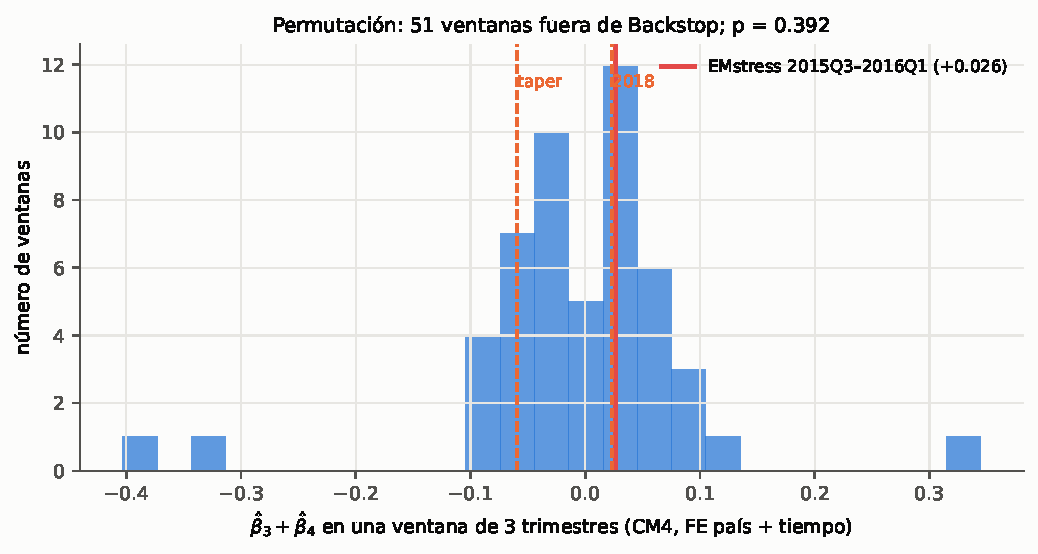
\includegraphics[width=\textwidth]{fig_permutacion_emstress_arb.pdf}\\
{\scriptsize Interacción con cada ventana de 3 trimestres en lugar de 2015--16.}
\end{columns}
\end{frame}

\begin{frame}{Anexo: Estrés conjunto y respaldo externo por país}
\centering
\footnotesize
\begin{adjustbox}{max width=\textwidth}
\begin{tabular}{l ccc c}
\toprule
\textit{Estrés conjunto} & Fragilidad alta & Cola alta & Las dos a la vez (extra) & Obs.\ conjuntas (esperadas) \\
\midrule
Terciles por país & $0{,}091^{*}$ & $0{,}186^{***}$ & $-0{,}077$ & 168 (87) \\
Cuartiles por país & $0{,}118^{***}$ & $0{,}125^{**}$ & $-0{,}122^{*}$ & 115 (49) \\
\midrule
\textit{Respaldo externo por país} & Fragilidad $\times$ acceso & Cola $\times$ acceso & Interacción $\times$ acceso & Obs.\ con acceso \\
\midrule
Muestra completa & $0{,}127$ & $0{,}002$ & $-0{,}004$ & 223 (6 países) \\
Dentro de las crisis globales & $0{,}063$ & $-0{,}018$ & $0{,}045^{**}$ & 54 de 109 \\
\bottomrule
\end{tabular}
\end{adjustbox}
\vspace{4pt}
\begin{itemize}\footnotesize
\item Los dos riesgos coinciden casi el doble de lo esperado por azar, pero juntos \textbf{no suman más} que por separado ($p$ \textit{wild} $0{,}23$).
\item Con acceso a un \textit{swap} de la Fed o a la línea flexible del FMI, la transmisión \textbf{no es menor} ($p$ \textit{wild} $0{,}90$; dentro de las crisis, $0{,}22$). No hay desacople.
\item \textit{Swap} de la Fed: Brasil y México. Línea flexible: México, Colombia, Polonia, Chile y Perú (2020Q2--2024Q2). El acceso no es exógeno.
\end{itemize}
\vspace{-2pt}
{\scriptsize *** $p<0{,}01$, ** $p<0{,}05$, * $p<0{,}10$ (Driscoll--Kraay).\par}
\end{frame}

\begin{frame}{Anexo: La elasticidad a la fragilidad no crece con el riesgo de cola}
\begin{columns}[c]
\column{0.52\textwidth}
\centering
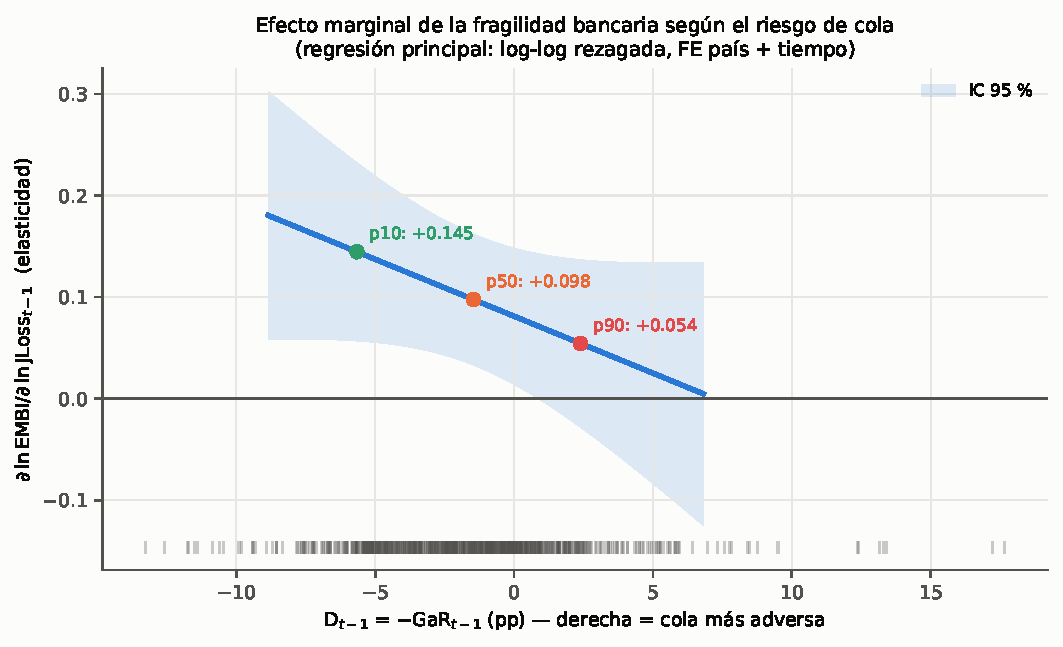
\includegraphics[width=\textwidth]{fig_efecto_marginal_lnlag.pdf}\\
{\scriptsize Elasticidad a la fragilidad según el riesgo de cola $D$.}
\column{0.46\textwidth}
\footnotesize
\begin{itemize}\setlength\itemsep{2pt}
\item La elasticidad \textbf{no crece} con el riesgo de cola: 0,145 $\to$ 0,098 $\to$ 0,054.
\item $\beta_3=-0{,}011$; IC 95\% con \textit{wild bootstrap}: $[-0{,}054;\,0{,}015]$.
\item El signo negativo es de Polonia (sin ella $+0{,}008$, $p=0{,}19$): no se lee como atenuación.
\item Aditivo en logaritmos es proporcional en pb: álgebra de la forma funcional.
\item \textbf{Señales débiles en contra}: fuera del piso de $\JLoss$ el riesgo de cola pesa $+7{,}5$ pb más ($p$ \textit{wild} $0{,}036$) con un umbral de 2\%, no en logaritmos; en cambios a cuatro trimestres en pb, $+0{,}358$ ($0{,}011$), ausente en logaritmos.
\end{itemize}
\end{columns}
\end{frame}

\begin{frame}{Anexo: Heterogeneidad: agrupación \textit{ex post}, exploratoria}
\centering
\footnotesize
\begin{adjustbox}{max width=\textwidth, max totalheight=0.44\textheight}
\begin{tabular}{l cc cc}
\toprule
 & \multicolumn{2}{c}{Log-log ($\beta_3$)} & \multicolumn{2}{c}{Niveles (pb)} \\
\cmidrule(lr){2-3}\cmidrule(lr){4-5}
 & Completa & Sin crisis & Completa & Sin crisis \\
\midrule
Núcleo (11 economías) & $0{,}011$ & $0{,}034^{***}$ & $0{,}78^{**}$ & $1{,}79^{***}$ \\
\quad $p$ \textit{wild cluster bootstrap} & $0{,}12$ & $0{,}015$ & $0{,}046$ & $0{,}002$ \\
\quad con seis controles & $0{,}004$ & $0{,}004$ & $0{,}53^{***}$ & $0{,}81^{***}$ \\
\quad $p$ \textit{wild} con controles & $0{,}39$ & $0{,}68$ & $0{,}042$ & $0{,}12$ \\
\quad \textit{leave-one-out} (rango) & $[0{,}002;0{,}015]$ & $[0{,}018;0{,}039]$ & $[0{,}27;0{,}93]$ & $[0{,}87;1{,}92]$ \\
\addlinespace
Polonia e India & $-0{,}059^{**}$ & $-0{,}118^{***}$ & $0{,}02$ & $-1{,}82^{**}$ \\
\bottomrule
\end{tabular}
\end{adjustbox}
\vspace{3pt}
\begin{alertblock}{Exploratorio}
\footnotesize El grupo se definió después de ver los datos; en logaritmos los controles lo absorben; y la variable que debía explicarlo, la participación extranjera en la deuda, no lo hace.
\end{alertblock}
\vspace{-2pt}
{\scriptsize\raggedright \textbf{Núcleo:} Brasil, Chile, China, Colombia, Filipinas, Indonesia, Malasia, México, Perú, Sudáfrica y Turquía. \textbf{Polonia e India:} agrupación \textit{ex post}. $\beta_3$: interacción de la especificación principal. *** $p<0{,}01$, ** $p<0{,}05$ (Driscoll--Kraay).\par}
\end{frame}

\begin{frame}{Anexo: Participación extranjera en la deuda: prueba preespecificada}
\begin{columns}[c]
\column{0.5\textwidth}
\centering
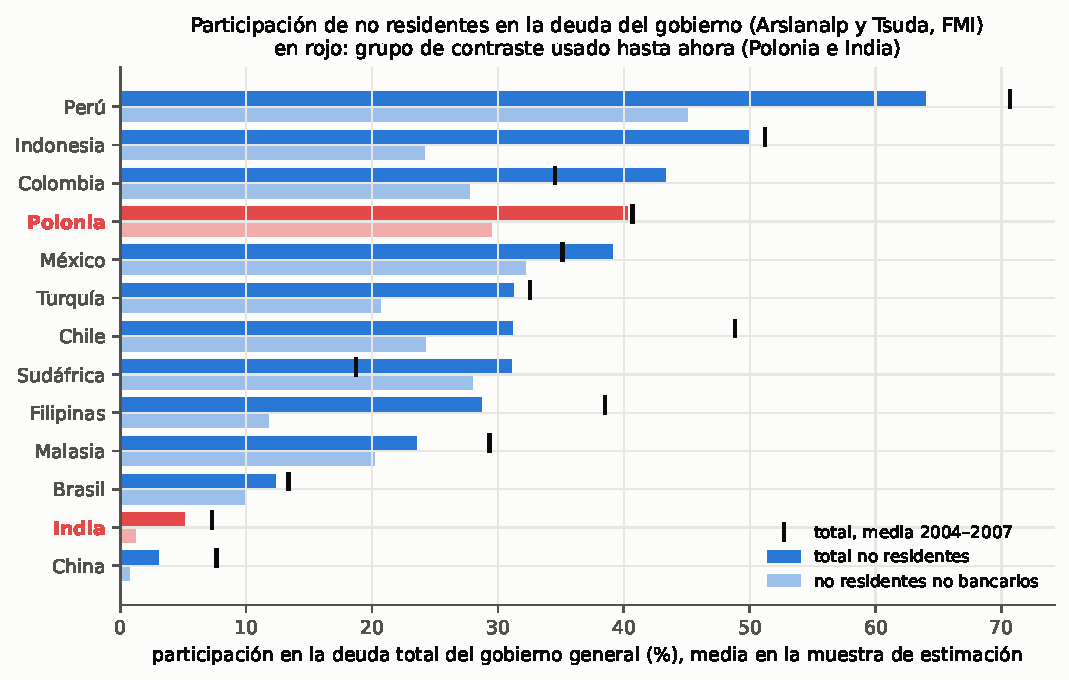
\includegraphics[width=\textwidth]{fig_participacion_extranjera.pdf}
\column{0.49\textwidth}
\centering
\footnotesize
\begin{adjustbox}{max width=\textwidth}
\begin{tabular}{l ccc}
\toprule
Familia primaria ($N=762$) & Coef. & $p$ \textit{wild} & $p$ Holm \\
\midrule
Fragilidad $\times$ participación & $0{,}037$ & $0{,}41$ & $1{,}00$ \\
Riesgo de cola $\times$ participación & $-0{,}001$ & $0{,}92$ & $1{,}00$ \\
Interacción $\times$ participación & $-0{,}006$ & $0{,}48$ & $1{,}00$ \\
\bottomrule
\end{tabular}
\end{adjustbox}

\vspace{3pt}
\raggedright
\begin{itemize}\setlength\itemsep{1pt}
\item \textbf{Preespecificada}: hipótesis, moderador y familia se fijaron antes de estimar.
\item Moderador: no bancos extranjeros en la deuda del gobierno, rezagado 4 trimestres (Arslanalp y Tsuda, FMI).
\item Ninguna pasa el criterio declarado (\textit{wild}). En pb la primera es sugerente: $+3{,}38$ (\textit{wild} $0{,}13$). Ausencia de evidencia, no evidencia de un cero.
\item \textbf{Polonia: 40\%} en manos de no residentes (4.ª de 13); India, 5\%; China, 3\%; Brasil, 12\%.
\end{itemize}
\end{columns}
\end{frame}

\begin{frame}{Anexo: Las reservas bajo escrutinio}
\centering
\footnotesize
\begin{adjustbox}{max width=\textwidth, max totalheight=0.47\textheight}
\begin{tabular}{l cc cc}
\toprule
 & \multicolumn{2}{c}{Logaritmos} & \multicolumn{2}{c}{Puntos básicos} \\
\cmidrule(lr){2-3}\cmidrule(lr){4-5}
Fragilidad $\times$ reservas/PIB (por desviación estándar de reservas) & Coef. & $p$ \textit{wild} & Coef. & $p$ \textit{wild} \\
\midrule
Reservas contemporáneas & $-0{,}247$ & $0{,}08$ & $-11{,}3$ & $0{,}04$ \\
Reservas rezagadas 4 trimestres & $-0{,}234$ & $0{,}05$ & $-10{,}9$ & $0{,}02$ \\
Reservas rezagadas 8 trimestres & $-0{,}190$ & $0{,}09$ & $-10{,}3$ & $0{,}06$ \\
\textbf{Sin Polonia} & $\mathbf{-0{,}084}$ & $0{,}30$ & $-9{,}5$ & $0{,}08$ \\
Reservas previas a la muestra & $-0{,}073$ & $0{,}30$ & $-4{,}3$ & $0{,}13$ \\
\textbf{Corrección de Holm} (3 componentes $\times$ 2 riesgos) & & $\mathbf{0{,}40}$ & & $\mathbf{0{,}22}$ \\
\midrule
\textit{Placebo:} fragilidad $\times$ cuenta corriente rezagada & $-0{,}113$ & $0{,}04$ & $-4{,}1$ & $0{,}06$ \\
\textit{Placebo:} fragilidad $\times$ tipo de cambio real rezagado & $+0{,}123$ & $0{,}02$ & $+3{,}6$ & $0{,}03$ \\
\bottomrule
\end{tabular}
\end{adjustbox}
\vspace{-1pt}
\begin{alertblock}{Lectura: exploratorio}
\footnotesize El coeficiente de la fragilidad es menor donde hay más reservas; es estable al rezagarlas y más firme en puntos básicos. Pero en logaritmos depende de Polonia, no pasa la corrección de Holm, otras variables macroeconómicas dan interacciones similares e implica una elasticidad negativa para el 23\% de las observaciones. No sustenta recomendar reservas.
\end{alertblock}
\end{frame}

\begin{frame}{Anexo: Robustez: qué depende de la muestra y qué no}
\centering
\small
\begin{adjustbox}{max width=\textwidth}
\begin{tabular}{ll}
\toprule
Ejercicio & ¿Cambia la conclusión? \\
\midrule
Agregar Argentina (14 países, 799 obs.) & No \\
\textit{Expected Shortfall} en vez de $\GaR$ & No \\
Sin el EMBI empalmado del FMI; desde 2010 & No \\
\textit{Spread} de cierre en vez del promedio & Niveles: no. Cambios: desaparece la precedencia \\
CDS soberano en vez del EMBI & Fragilidad: no. Riesgo de cola: deja de ser significativo \\
Excluir cada país: amplificación & No aparece; el signo negativo es de Polonia \\
Excluir cada país: cada riesgo & Sí: Turquía (fragilidad) y Polonia (riesgo de cola) \\
Todo en puntos básicos & Más favorable, pero no resiste el \textit{wild bootstrap} \\
\bottomrule
\end{tabular}
\end{adjustbox}
\end{frame}

\begin{frame}{Anexo: logaritmos vs.\ niveles}
\centering
\footnotesize
\begin{tabular}{llcc}
\toprule
Forma & Regresores & Muestra completa & Sin crisis \\
\midrule
Niveles (pb) & contemporáneos & $+0{,}177$ & $+1{,}183^{***}$ \\
 & rezagados & $+0{,}246$ & $+1{,}294^{***}$ \\
\addlinespace
Logaritmos & contemporáneos & $-0{,}0145^{**}$ & $-0{,}0052$ \\
 & rezagados (principal) & $-0{,}0112$ & $+0{,}0045$ \\
\bottomrule
\end{tabular}
\vspace{6pt}
\begin{itemize}\footnotesize
\item Lo que elimina la interacción es el logaritmo, no el rezago.
\item Prueba PE: rechaza niveles frente a logs ($t=-3{,}56$), no al revés ($t=1{,}04$).
\item Box--Cox: $\hat\lambda=0{,}44$ [0,38; 0,50]: forma intermedia.
\end{itemize}
\end{frame}

\begin{frame}{Anexo: Argentina}
\centering
\small
\begin{tabular}{lcc}
\toprule
M4, EF país + tiempo & Sin Argentina & Con Argentina \\
\midrule
$\beta_1$ / $\beta_2$ & $0{,}0985^{***}$ / $0{,}0324^{**}$ & $0{,}0964^{***}$ / $0{,}0326^{**}$ \\
$\beta_3$ & $-0{,}0112$ ($p=0{,}11$) & $-0{,}0082$ ($p=0{,}28$) \\
\textit{Backstop} $\beta_3+\beta_4$ & $-0{,}0146$ ($p=0{,}03$) & $-0{,}0120$ ($p=0{,}03$) \\
\textit{EMstress} EF país+tiempo & $0{,}026$ ($p=0{,}08$) & $0{,}024$ ($p=0{,}13$) \\
$N$ & 765 & 799 \\
\bottomrule
\end{tabular}
\vspace{6pt}

\footnotesize Su $\GaR$ se estimó sin el bloque de tasas y con una ventana más corta: por eso es robustez.
\end{frame}

\begin{frame}[allowframebreaks]{Referencias principales}
\scriptsize
\begin{itemize}
\item Acharya, V., Drechsler, I., \& Schnabl, P. (2014). A Pyrrhic Victory? Bank Bailouts and Sovereign Credit Risk. \textit{Journal of Finance}, 69(6), 2689--2739.
\item Adrian, T., Boyarchenko, N., \& Giannone, D. (2019). Vulnerable Growth. \textit{American Economic Review}, 109(4), 1263--1289.
\item Arslanalp, S., \& Tsuda, T. (2014). Tracking Global Demand for Emerging Market Sovereign Debt. \textit{IMF Working Paper} 14/39 (base actualizada a mayo de 2026).
\item Bernanke, B., Gertler, M., \& Gilchrist, S. (1996). The Financial Accelerator and the Flight to Quality. \textit{Review of Economics and Statistics}, 78(1), 1--15.
\item Calvo, G., Leiderman, L., \& Reinhart, C. (1996). Inflows of Capital to Developing Countries in the 1990s. \textit{Journal of Economic Perspectives}, 10(2), 123--139.
\item Cameron, A. C., Gelbach, J. B., \& Miller, D. L. (2008). Bootstrap-Based Improvements for Inference with Clustered Errors. \textit{Review of Economics and Statistics}, 90(3), 414--427.
\item Chari, A., Garcés, F., Martínez, J. F., \& Valenzuela, P. (2024). Sovereign Credit Spreads, Banking Fragility, and Global Factors. \textit{Journal of Financial Stability}, 72, 101235.
\item Driscoll, J. C., \& Kraay, A. C. (1998). Consistent Covariance Matrix Estimation with Spatially Dependent Panel Data. \textit{Review of Economics and Statistics}, 80(4), 549--560.
\item Duffie, D., \& Singleton, K. (1999). Modeling Term Structures of Defaultable Bonds. \textit{Review of Financial Studies}, 12(4), 687--720.
\item Edwards, S. (1984). LDC Foreign Borrowing and Default Risk. \textit{American Economic Review}, 74(4), 726--734.
\item Farhi, E., \& Tirole, J. (2018). Deadly Embrace: Sovereign and Financial Balance Sheets Doom Loops. \textit{Review of Economic Studies}, 85(3), 1781--1823.
\item Goldsmith-Pinkham, P., Sorkin, I., \& Swift, H. (2020). Bartik Instruments: What, When, Why, and How. \textit{American Economic Review}, 110(8), 2586--2624.
\item Hansen, B. E. (1999, 2000). Threshold Effects in Non-Dynamic Panels / Sample Splitting and Threshold Estimation.
\item Hilscher, J., \& Nosbusch, Y. (2010). Determinants of Sovereign Risk. \textit{Review of Finance}, 14(2), 235--262.
\item Longstaff, F., Pan, J., Pedersen, L., \& Singleton, K. (2011). How Sovereign Is Sovereign Credit Risk? \textit{AEJ: Macroeconomics}, 3(2), 75--103.
\item Miranda-Agrippino, S., \& Rey, H. (2022). The Global Financial Cycle. \textit{Handbook of International Economics}, Vol.\ 6.
\item Ossandon Busch, M. et al.\ (2022). Growth at Risk: Methodology and Applications in an Open-Source Platform (CEMLA).
\item Uribe, M., \& Yue, V. Z. (2006). Country Spreads and Emerging Countries: Who Drives Whom? \textit{Journal of International Economics}, 69(1), 6--36.
\end{itemize}
\end{frame}

\end{document}
